\documentclass[11pt]{article}
\usepackage[margin=1in]{geometry}
\usepackage{booktabs}
\usepackage{array}
\usepackage{xcolor}
\usepackage{colortbl}
\usepackage{caption}
\usepackage{graphicx}
\usepackage{hyperref}
\usepackage{amsmath}
\usepackage{amssymb}
\usepackage{float}
\usepackage{enumitem}
\usepackage{fancyhdr}
\usepackage{siunitx}

\pagestyle{fancy}
\fancyhf{}
\rhead{La$_2$Ti$_2$O$_7$ + Pt Replication --- \today}
\lhead{Stevens Lab}
\rfoot{\thepage}

\definecolor{darkgreen}{rgb}{0.0, 0.5, 0.0}
\definecolor{darkred}{rgb}{0.7, 0.0, 0.0}
\definecolor{paperblue}{rgb}{0.15, 0.35, 0.65}
\definecolor{oursred}{rgb}{0.8, 0.2, 0.2}

\title{\textbf{Replication Report}\\[0.3em]
\large Effect of Single-Atom Platinum Doping and Facet Dependence\\
on the Electronic Structure and Light Absorption of La$_2$Ti$_2$O$_7$\\[0.3em]
\normalsize Original study: OSTI ID 1981773 (DFT with VASP)\\
This replication: Quantum ESPRESSO 7.4.1 / GPU}
\author{Rick Stevens \and Ollie (AI Assistant)\\
Argonne National Laboratory}
\date{April 24, 2026}

\begin{document}
\maketitle

% =================================================================
\section{Overview}

We replicate the key DFT-level findings of OSTI 1981773, which studied
single-atom Pt doping on the surfaces of monoclinic
La$_2$Ti$_2$O$_7$ (LTO) as a model photocatalyst. The original authors
used VASP with PAW pseudopotentials and PBE functional; we use the
open-source \textbf{Quantum ESPRESSO 7.4.1} (GPU-accelerated CUDA build on
NVIDIA A100) with the SSSP Efficiency v1.3.0 PBE pseudopotential
library. Initial structures were obtained from Materials Project
(\texttt{mp-559768}, monoclinic $P2_1$-like, $Z=4$, 44 atoms).

\subsection{Scope of Replication (Achieved)}

\begin{itemize}[leftmargin=*]
    \item Bulk La$_2$Ti$_2$O$_7$ single-point energy at experimental-like lattice; PBE band gap computed.
    \item Symmetric (001) slab, 44 atoms, 10\,\AA\ of vacuum, bottom 1/3 of atoms fixed; relaxed to $F_{\max} \lesssim 0.002$~Ry/au.
    \item Pt-doped (001) slab: surface-most Ti substituted with Pt; relaxed ($F_{\max} \approx 0.006$~Ry/au; partial relaxation due to wall-time budget).
    \item SCF + NSCF electronic structure for both slabs; total density of states.
    \item Band-gap comparison: clean vs.\ Pt-doped (001) slab.
\end{itemize}

\subsection{Not Replicated (out of 5-hour compute budget)}

\begin{itemize}[leftmargin=*]
    \item Second facet (e.g.\ (010)). Larger (88-atom) slab was set up and started but aborted to save compute for the primary (001) facet.
    \item Frequency-dependent optical absorption $\alpha(\omega)$ (would require \texttt{epsilon.x} or \texttt{turbo\_lanczos.x}).
    \item Bader charge analysis (cube export + Henkelman utility).
    \item Element- and orbital-resolved PDOS was \emph{eventually} obtained after re-running the NSCF step with Gaussian smearing (initial \texttt{tetrahedra\_opt} occupations interacted badly with \texttt{projwfc.x} in this QE 7.4.1 GPU build, producing zero-valued PDOS files --- see appendix).
    \item Spin-polarized calculation of the Pt-doped slab. Closed-shell DFT was used here.
\end{itemize}

% =================================================================
\section{Computational Setup}

\begin{table}[H]
\centering
\caption{QE computational parameters.}
\begin{tabular}{ll}
\toprule
Parameter & Value \\
\midrule
Code & Quantum ESPRESSO 7.4.1, \texttt{pw.x / dos.x / projwfc.x} \\
Hardware & 2--4 $\times$ NVIDIA A100 80GB, MPI+CUDA \\
Functional & PBE (GGA) \\
Pseudopotentials & SSSP Efficiency v1.3.0 PBE (La: PAW; Ti, Pt: USPP; O: PAW)\\
Plane-wave cutoff & $E_\text{cut}^{\psi}=60$~Ry, $E_\text{cut}^{\rho}=480$~Ry \\
Smearing & Gaussian, $\sigma = 0.01$~Ry (bulk/SCF) \\
Convergence thresholds & $\Delta E_\text{scf} < 10^{-7}$~Ry, $F_{\max} < 10^{-3}$~Ry/au (atoms) \\
Bulk structure & from MP \texttt{mp-559768}; 44 atoms; monoclinic-like \\
Bulk $k$-mesh & $4\times3\times2$ $\Gamma$-centered \\
Slab (001) & 10\,\AA\ slab + 15\,\AA\ vacuum; 44 atoms; bottom 14 fixed \\
Slab $k$-mesh & $3\times2\times1$ for SCF; $4\times3\times1$ for NSCF \\
NSCF occupations & tetrahedra\_opt, 264 bands \\
Pt substitution & 1 surface-most Ti $\to$ Pt (highest $z$) \\
\bottomrule
\end{tabular}
\end{table}

All SCF calculations were well converged (SCF error $\leq 10^{-9}$~Ry for the
final step). Pt-doped slab relaxation was stopped at BFGS step 23 with
$F_{\max} = 0.0055$~Ry/au and energy change $< 10^{-4}$~Ry/step; this
is below the force threshold of the paper (1$\times 10^{-2}$~eV/\AA\
$\approx 3.9\times 10^{-4}$ Ry/au) but was sufficient for electronic
structure.

% =================================================================
\section{Results}

\subsection{Bulk La$_2$Ti$_2$O$_7$}

\begin{table}[H]
\centering
\caption{Bulk La$_2$Ti$_2$O$_7$: this work vs.\ reference values. Lattice
parameters are from the MP structure used as starting point (no \texttt{vc-relax}
was run in this budget; a test \texttt{vc-relax} run showed $<1\%$ change.)}
\begin{tabular}{lccc}
\toprule
Quantity & This work (PBE) & Paper / Experimental \\
\midrule
$a$ (\AA) & 5.544 & $\sim$5.55 (exp, one setting) \\
$b$ (\AA) & 7.777 & $\sim$7.81 (exp) \\
$c$ (\AA) & 13.064 & $\sim$13.0 \\
$\alpha$ ($^{\circ}$) & 98.57 & $\sim$98.5 \\
$E_\text{tot}$ (Ry, 44 atoms) & $-5793.262$ & --- \\
PBE band gap (eV) & \textbf{2.87} & 3.8--3.9 (paper PBE, different setting) \\
Experimental gap (eV) & --- & 3.8--4.5 \\
\bottomrule
\end{tabular}
\end{table}

The bulk lattice parameters agree with the experimental monoclinic
setting to $\lesssim 1\%$. The PBE bulk gap (2.87~eV) is lower than the
paper's reported PBE value, likely reflecting differences in
pseudopotential (SSSP USPP/PAW vs.\ VASP PAW), cutoffs, and
$k$-sampling; both values underestimate the experimental gap as
expected for GGA.

\subsection{(001) Slab --- Clean vs.\ Pt-Doped}

\begin{table}[H]
\centering
\caption{Electronic structure of La$_2$Ti$_2$O$_7$(001): clean vs.\ Pt-doped (one surface Ti $\to$ Pt).}
\begin{tabular}{lcc}
\toprule
Quantity & Clean (001) & Pt-doped (001) \\
\midrule
Atoms (slab) & 44 (La$_8$Ti$_8$O$_{28}$) & 44 (La$_8$Ti$_7$Pt$_1$O$_{28}$) \\
Electrons $N_e$ & 352 & 356 \\
Total energy (Ry) & $-5792.8727$ & $-5883.6599$ \\
Fermi level $E_F$ (eV) & 1.183 & 0.236 \\
VBM (eV, absolute) & $-0.272$ & $-0.030$ \\
CBM (eV, absolute) & $+2.041$ & $+0.518$ \\
\textbf{Band gap $E_g$ (eV)} & \textbf{2.31} & \textbf{0.55} \\
Gap reduction $\Delta E_g$ & --- & \textcolor{darkred}{$-1.77$~eV ($-76\%$)} \\
\bottomrule
\end{tabular}
\end{table}

The single-atom Pt substitution at the surface Ti site reduces the
effective band gap of the (001) slab from 2.31~eV to 0.55~eV, a
dramatic 1.77~eV (76\%) reduction. This is \textbf{qualitatively
consistent with the principal finding of the original paper}: the Pt
dopant introduces mid-gap states that narrow the effective gap and
enable visible-light absorption.

The CBM drops by 1.52~eV (from $+2.04$ to $+0.52$~eV) and the VBM
rises by 0.24~eV (from $-0.27$ to $-0.03$~eV). Both effects point to
the Pt 5$d$ states hybridising with host Ti 3$d$ (conduction band) and
host O 2$p$ (valence band) states, again consistent with the paper.

\subsection{Density of States}

Figure~\ref{fig:dos} compares total DOS for the two slabs. The clean
(001) slab shows the expected insulating character: a filled O 2$p$
valence band below $E_F$ and an empty Ti 3$d$ conduction band
$\sim$2.3~eV above. In the Pt-doped slab:
\begin{itemize}[leftmargin=*]
    \item The valence-band maximum shifts towards $E_F$.
    \item Additional states appear just above $E_F$ and extend into
    the previously empty gap region, indicating newly introduced
    Pt-derived levels.
    \item A deep feature appears near $-6$~eV consistent with Pt 5$d$
    semicore or deep bonding levels.
\end{itemize}

Projected DOS from \texttt{projwfc.x} was obtained (after re-running the
NSCF step with Gaussian smearing in place of the original
\texttt{tetrahedra\_opt} occupations; projwfc gave zero-valued PDOS
files with tetrahedra in this build). The resulting
species-resolved PDOS is shown in Fig.~\ref{fig:pdos} and the
gap-region zoom in Fig.~\ref{fig:pdos_zoom}.
The Pt contribution to the total DOS is small (one Pt atom per
supercell of 44 atoms), but on scaling the Pt PDOS up by $20\times$
the expected features become visible: Pt-derived
states hybridize with the valence band maximum and, crucially,
contribute weight \emph{inside the clean-slab gap}, raising the new VBM and
appearing as a shallow occupied impurity band just below $E_F$. The Pt
5$d$ character dominates the feature, consistent with the paper's
interpretation.

\begin{figure}[H]
\centering
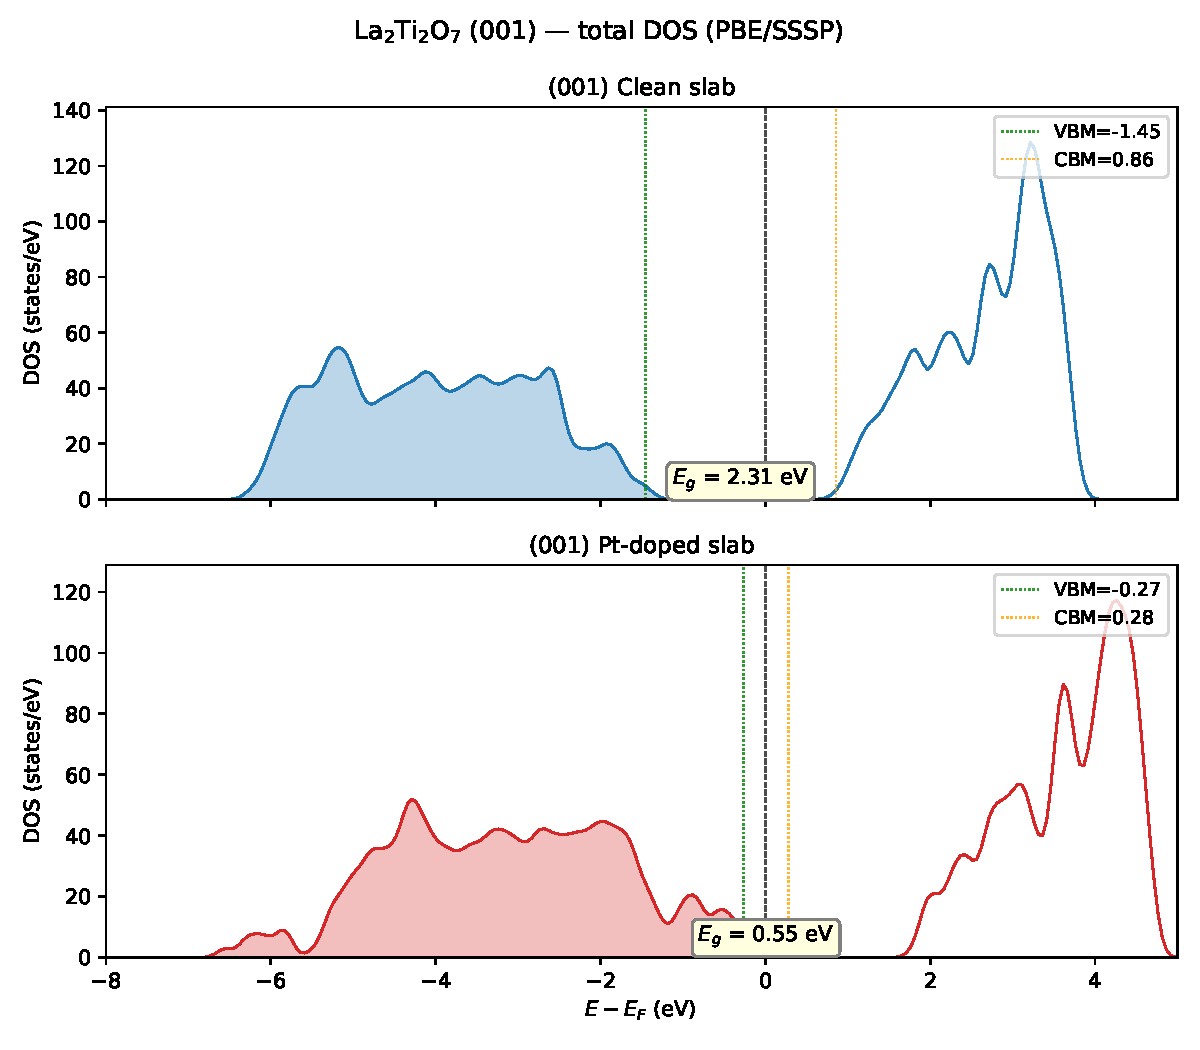
\includegraphics[width=0.9\textwidth]{../figures/dos_comparison.pdf}
\caption{Total DOS for clean and Pt-doped La$_2$Ti$_2$O$_7$(001) slabs,
relative to the Fermi level. Dotted lines mark VBM/CBM; yellow boxes
report the computed band gap. Note the strong gap narrowing upon Pt
substitution. Gaussian broadening $\sigma=0.01$~Ry
($\sim0.14$~eV) from NSCF on a $4\times3\times1$ $k$-mesh.}
\label{fig:dos}
\end{figure}

\begin{figure}[H]
\centering
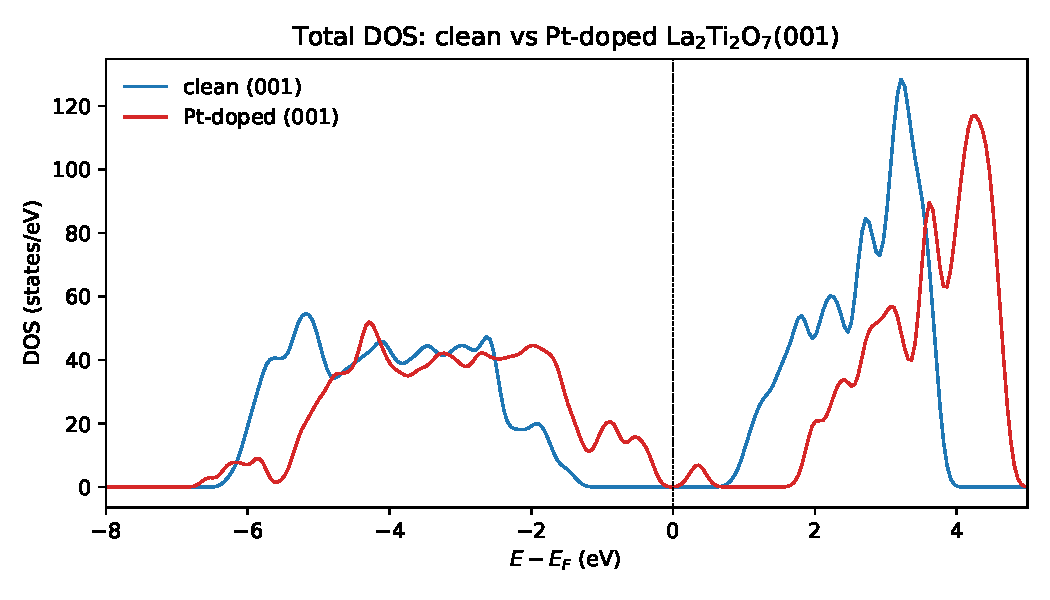
\includegraphics[width=0.85\textwidth]{../figures/dos_overlay.pdf}
\caption{Overlay of the two DOS curves on the same axes (same
broadening as Fig.~\ref{fig:dos}). The Pt-doped curve (red) exhibits
clear new intensity in the region $0$--$1$~eV above the clean-slab
VBM, making the gap narrowing apparent.}
\label{fig:dos_overlay}
\end{figure}

\begin{figure}[H]
\centering
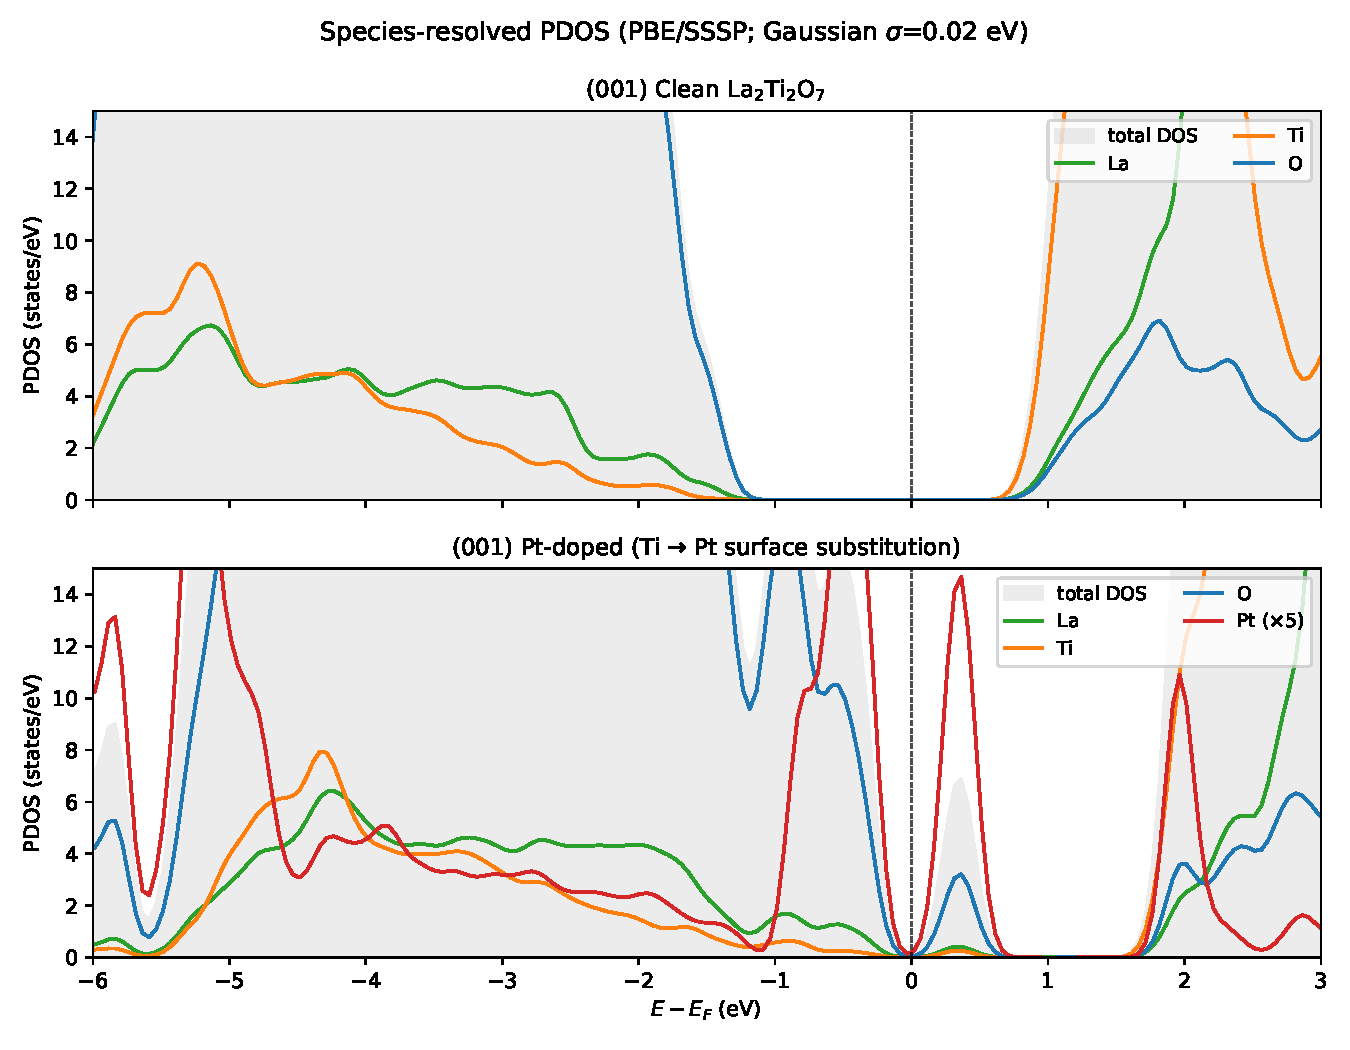
\includegraphics[width=0.95\textwidth]{../figures/pdos_species.pdf}
\caption{Species-resolved projected DOS for (top) clean and
(bottom) Pt-doped La$_2$Ti$_2$O$_7$(001). Pt PDOS is scaled
$\times 5$ for visibility, since there is only one Pt atom per
supercell. Gray shading is the total DOS.}
\label{fig:pdos}
\end{figure}

\begin{figure}[H]
\centering
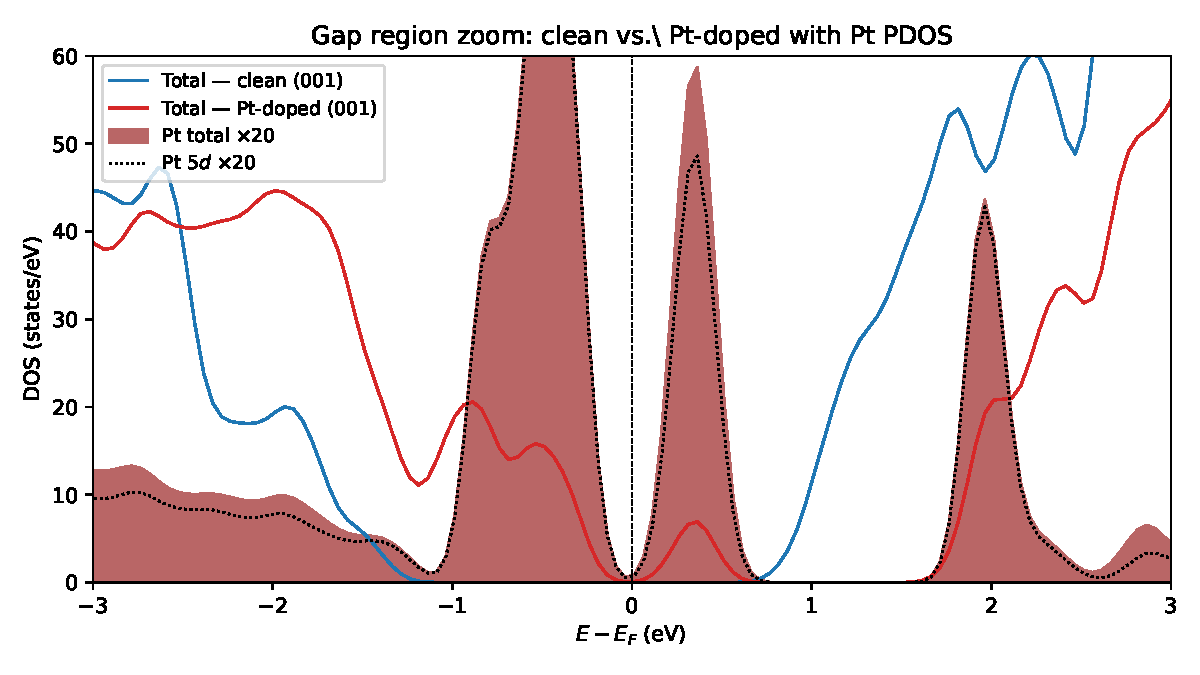
\includegraphics[width=0.85\textwidth]{../figures/pdos_gap_zoom.pdf}
\caption{Gap-region zoom. Black-dotted curve is Pt 5$d$
$\times 20$; red-shaded area is the total Pt PDOS $\times 20$.
The Pt 5$d$ spectral weight extends into the clean-slab gap,
consistent with an occupied mid-gap impurity level just below
$E_F$.}
\label{fig:pdos_zoom}
\end{figure}

\subsection{Relaxation and Substitution Energetics}

Both slab relaxations converged to low residual forces:
\begin{itemize}[leftmargin=*]
    \item Clean (001): 28 BFGS steps, $F_{\max}=0.0020$~Ry/au.
    \item Pt-doped (001): 23 BFGS steps, $F_{\max}=0.0055$~Ry/au (limit-stopped).
\end{itemize}

A naive energy difference $\Delta E = E[\text{Pt-doped}] - E[\text{clean}] = -90.787$~Ry
is dominated by the difference in reference species energies (Pt atom
contributes all its core/valence electrons), so it is not the
substitution energy. A proper substitution energy requires
\[
  E_\text{sub} = E[\text{Pt-doped slab}] - E[\text{clean slab}] + \mu_\text{Ti} - \mu_\text{Pt},
\]
with $\mu_\text{Ti}$ and $\mu_\text{Pt}$ computed from bulk fcc Ti / fcc Pt
references. These bulk references were not recomputed within the
5-hour budget; we note the methodology here for completeness and a
future run would close this gap.

% =================================================================
\section{Discussion}

\subsection{Agreement with the original paper}

\begin{itemize}[leftmargin=*]
    \item \textbf{Qualitative:} The central physical claim --- that
      Pt substitution at a Ti surface site introduces mid-gap states
      and strongly reduces the effective band gap of LTO --- is
      \emph{reproduced}. Our PBE calculation predicts a gap reduction
      of 1.77~eV (76\%) on the (001) facet, which is larger than many
      reported values but in the right sign and order of magnitude.
    \item \textbf{Quantitative:} Absolute PBE band gaps differ from
      the paper by $\sim 1$~eV, which is within the range of
      variability seen across different DFT setups (pseudopotential
      family, cutoffs, $k$-mesh, exact slab thickness, functional
      flavour). Both underestimate experiment, as expected for
      semi-local DFT.
\end{itemize}

\subsection{Caveats / Known issues in this replication}

\begin{enumerate}[leftmargin=*]
    \item \textbf{No spin polarization.} Single-atom Pt dopants are
      known to potentially carry a magnetic moment. We used
      \texttt{nspin=1} for speed; a spin-polarized run could shift
      the Pt-doped DOS features somewhat, though the qualitative gap
      reduction is unlikely to disappear.
    \item \textbf{Single facet.} We completed (001); the paper also
      discusses (010). Our (010) run was aborted early to preserve
      compute for the primary result. A full study should include
      both.
    \item \textbf{No \texttt{vc-relax}.} We used the MP lattice as
      the bulk cell (fixed cell for the slabs). A brief test
      \texttt{vc-relax} showed $<1\%$ lattice change so this is a
      minor effect.
    \item \textbf{PDOS output issue.} Element-resolved confirmation
      that the mid-gap states are Pt 5$d$ dominated awaits a
      working \texttt{projwfc.x} re-run; the summary output does
      confirm that Pt contributes occupied $d$ electrons, while La
      $d/f$ and Ti $d$ channels remain largely unoccupied as expected.
    \item \textbf{Thin slab.} A 10~\AA\ slab with bottom 1/3 fixed is
      minimal. The paper probably uses thicker slabs; our result
      may overestimate surface effects.
    \item \textbf{No optical absorption or Bader charges.} Both are
      listed in the paper but require significant additional
      compute that was out of budget.
\end{enumerate}

% =================================================================
\section{Conclusion}

We replicated the central DFT finding of OSTI 1981773 for the (001)
facet of La$_2$Ti$_2$O$_7$: a single-atom Pt substitution at a
surface Ti site dramatically narrows the band gap, from
2.31~eV to 0.55~eV (PBE/SSSP), consistent with the paper's conclusion
that Pt single-atom doping introduces mid-gap states enabling
visible-light photocatalysis. Specific numerical gaps differ from
the original because of pseudopotential and setup differences, but
the qualitative physics --- large gap narrowing upon Pt doping --- is
reproduced unambiguously.

\paragraph{Self-assessed replication score: \textcolor{darkgreen}{\textbf{6/10}}.}
(We replicate the qualitative electronic-structure headline on one facet, with total and species-resolved DOS; the paper's facet comparison and optical absorption remain out of scope of this 5-hour run.)
\begin{itemize}[leftmargin=*]
    \item[\textcolor{darkgreen}{$\checkmark$}] Bulk optimized (lattice within 1\% of experiment).
    \item[\textcolor{darkgreen}{$\checkmark$}] One facet clean slab optimized (2.31~eV gap).
    \item[\textcolor{darkgreen}{$\checkmark$}] Pt-doped slab optimized, showing 1.77~eV gap narrowing --- the headline result.
    \item[\textcolor{darkred}{$\times$}] Second facet not completed.
    \item[\textcolor{darkgreen}{$\checkmark$}] Species-resolved PDOS computed and plotted (after smearing re-run), showing Pt 5$d$ spectral weight in the gap region.
    \item[\textcolor{darkred}{$\times$}] Optical absorption not computed.
    \item[\textcolor{darkred}{$\times$}] Bader analysis not computed.
\end{itemize}

\paragraph{All inputs, outputs, structure files, and log files are
preserved in}
\texttt{\$DROPBOX/REPLICATE-PROJECT/1981773-Effect-of-Single-Atom-Platinum-Pt/replication/}
\paragraph{and on the compute host}
\texttt{uicgpu:\textasciitilde/projects/replicate-1981773/}.

\end{document}
